\chapter{Human Ability of Counting Concurrent Sources}

TODO... Write a proper chapter introduction.

\begin{itemize}
  \item why is counting interesting
  \item are we calling it count estimation and not counting?
  \item why can't humans count for a high number of sources?
  \item counting on music signals in ill defined music signals lack a proper source definition.
\end{itemize}

\section{Experiments on Instrument Count Estimation}

Decomposing music into its original audio sources can be a challenging task. Source separation methods can be analyzed how well they perform mathematically, but a human versus machine comparison is cumbersome because measurement of the human separation performance is problematic. One can easily evaluate if humans can detect the number of sources in a mixture of several sources. However, there are indications that even for this task, humans tend to fail if more than three sources are present at the same time \cite{huron89}. Therefore, we want to take a first step by designing an experiment where we focus on polyphonic music of inhomogeneous timbre, where the question is: What is the number of instruments humans can estimate correctly? Several results are addressed in this paper including a possible upper limit of the number of perceived instruments, but also if one can see significant differences in performance of musicians compared to non-musicians. Such results can be used in auditory modeling or as a pre-processing step for source separation algorithms.
This paper presents the results of an experiment, a detailed description of the stimuli and the statistical methods that were used.

\subsection{Related Work}
The perception of concurrent sound sources has been analyzed on different scales so far. Bregman's and McAdams' \cite{mcadams79} auditory stream theory can be seen as an analytical way of describing how sound events are perceived by the human auditory system. Unfortunately, it is difficult to model professionally produced music by auditory stream models because of its high complexity. As described by Wang \cite{wang2006} there exist several algorithms to estimate the actual number of sources. However, none of them is motivated to model the perceived number of musical sources. Kashino et. al \cite{kashino1995} addresses the questions for concurrent speakers in a ``cocktail party'' like environment and found an upper limit of three voices humans can perceive. When the focus shifts to musical instruments as sources, research has to take concepts from musicology into account. Huron \cite{huron89} was the first who addressed this question in 1989 at a musically meaningful level. Huron asked for the number of voices within a piece of music, where by voices in musicology one can define it as a line of sound or note events (See \cite{cambouropoulos2008voice} for further definitions). Huron determined by experimental results that the number of correctly identified voices is up to three. Later in 1996, Reuter \cite{reuter96} has analyzed how combinations of different instruments are perceived which sets the focus on different instrumentation and not on denumerability.

\subsection{Experiment}
For the purpose of gaining more knowledge in understanding the human perception of multiple present instruments, an experiment was conducted. Huron selected voices from organ pieces only. We wanted to address the more general case where voices are played by different instruments. Therefore we used a method between musicology and auditory stream analysis to address this question. As we set our focus mainly on comparison between musicians and non-musicians, our experiment was designed so that it respects the fact that the latter have only limited musical background.

Although it might be interesting to have direct comparison with Huron's experiment, we agree that expanding the methods to an inhomogeneous timbre case is error prone. One reason is that there is reasonable doubt about the non-musicians understandings in terms of how a voice is defined. This is why we choose a trade-off with a more simplified experiment where we asked for the number of instruments instead of voices. Also whereas Huron \cite{huron89}  excluded subjects from his experiment because of their lower performance, we compared the results of both groups.

\subsection{Stimuli}

The selection of music items is crucial for our experiment setup. Usually music recordings have no ground truth metadata available to determine the actual number of instruments. Using annotated music like that from the RWC database \cite{rwc} fulfills this requirement but lacks the possibility to remix, attenuate or suppress specific sources. This is important so that the experiment consists of equally grouped stimuli. Instead of the original RWC recordings, the annotated MIDI data itself was used as prototypes for the stimuli.

To make the counting task less ambiguous for the subjects, the instrumentation needs to be mostly constant during the music piece. Therefore we calculated an ``instrumental stationarity'' measure. The annotated MIDI files from \cite{rwc} were converted into piano roll representations for each instrument channel. This representation was then converted into a binary \emph{instrumentation activity matrix} $\mathbf{I}_{AM}\lbrack \mathbf{\underline{k}}_1 \vert \mathbf{\underline{k}}_2 \vert  ... \vert \mathbf{\underline{k}}_N \rbrack \in \{0,1\}$, where at each discrete time instant $i$ a vector $\mathbf{\underline{k}}_i$ indicates which instruments are active. The aim is then to select frames of length $N$ which are stationary by means of changes in instrumentation and activity. To get many items with a high instruments count, the maximum number of instruments within a frame was stored in a binary mask $\mathbf{\underline{k}}_{max}$ which was compared with all $\mathbf{\underline{k}}_{i=1...N}$ so that $(\vert\mathbf{\underline{k}}_{i} \oplus \mathbf{\underline{k}}_{max}\vert \leq 1) \lor (\mathbf{\underline{k}}_{i} = \underline{0})$. The resulting binary vector was smoothed with an averaging kernel of size $N$. By peak picking we got a list of possible candidates which contained a high stationarity in instrumentation.
Further the RWC files were filtered a priori to exclude items dominated by electronic instruments or singing voice. Table~\ref{tab:items} presents the selected 12 items representing pairs of one to six simultaneously present instruments. Each item is around seven seconds long. By cutting at note offsets we varied the lengths of the items to make it semantically more meaningful. Six items (notated as RM-C***) belong to the classical western music genre whereas the other items are of mixed genre.

The MIDI excerpts were humanized and rendered by a sequencer software utilizing state-of-the-art commercial sampling products into WAV files. The rendered files were processed with convolutive reverb to match the original recordings. In informal listening tests the quality of the renderings was evaluated. In addition, participants did not give negative feedback about the artificialness of the items during the laboratory experiment. Additionally a loudness normalization was applied according to EBU-R128\cite{EBU2011}. To avoid spatial cues the files were downmixed to mono at 16~bit/44.1~kHz.


\begin{table}[htb]
\center
\tiny
\begin{tabular}{c|r@{.}l|r@{.}l|p{3.8cm}|c}
\toprule[1.5pt]
RWC~ID & \multicolumn{2}{c}{Start~[s]} & \multicolumn{2}{c}{Dur.~[s]} & Instrumentation & $\sum$\\
\midrule
\hline
J021 & 46 & 5 & 6 & 6 & Piano, Contrabass~(pizz.) and Trumpet & 3\\
\hline
\hline
C001 & 0&0 & 9&0 & Bassoon & 1  \\
G047 & 35&3 & 8&3 & Violoncello & 1 \\
\hline
C016 & 0&9 & 7&6 & Viola and Violoncello & 2\\
G068 & 132&4 & 6&6 & Violin and Flute &  2\\
\hline
C018 & 240&4 & 5&4 & French~Horn, Piano and Violin & 3\\
G046 & 0&3 & 7&9 & Contrabass, Piano and Violoncello & 3\\
\hline
C013 & 5&6 & 6&0 & Flute, Viola, Violin and Violoncello & 4\\
G036 & 0&0 & 6&5 &  Acoustic~Guitar, Electric~Bass, Piano  and Violin & 4\\
\hline
C012 & 112&0 & 6&0 & Contrabass, Flute, Viola, Violin and  Violoncello & 5\\
G037 & 67&1 & 7&0 & Acoustic~Guitar, Contrabass~(pizz.), Flute, Piano and Tenor~Sax & 5\\
\hline
C001 & 147&8 & 6&0 & Bassoon, Clarinet, Contrabass, French~Horn, Oboe and Violin & 6\\
G028 & 17&5 & 6&5 & Electric~Bass, Electric~Guitar, Flute, Piano, Trombone and Trumpet & 6\\
\hline
\bottomrule[1.5pt]
\end{tabular}
\caption{Selected items from the RWC Music Database \cite{rwc}. Item \emph{J021**} is used as training item.}
\label{tab:items}
\end{table}

\subsection{Large Scale Study}

For many types of music perception experiments such as estimating the number of instruments, it is essential that the selected participants represent a large population. As recent research in cross-cultural music perception and cognition reveals: The perception of music is dependent on the origin of people\cite{Stevens2012}. Besides the cultural background, other aspects like their profession might have an influence when estimating the number of instruments being played back, e.~g. musicians might recognize instruments much more easily since they are in touch with instruments in their everyday life. One of the advantages of Internet experiments (also called web-based experiments or web experiments) is that it is easier to gather participants with different backgrounds and from different regions than in laboratory experiments. For a summary of benefits and disadvantages of Internet experiments see \cite{Reips2002}. In music perception a major argument against Internet experiments is that there is no control about the environment. With the spreading of mobile devices with Internet connections this argument becomes more apparent, since the environment of the participants can range from a quiet place at home to a noisy place outside.

By comparing the results of the Internet experiment presented in this paper to the results of the same experiment but previously conducted in a controlled environment\cite{Stoter2013}, we contribute to answering the research question, whether the Internet can be used for experiments in music perception. Furthermore, subpopulations like headphones-users and loudspeaker-users are examined whether they lead to more reliable responses.

Participation in the experiment was done by visiting the experiment's website\footnote{{\scriptsize\url{http://www.audiolabs-erlangen.com/experiments/wice/}}}. The experiment was promoted in mailing lists, forums, social networks and by personal invitations. Most of the forums and mailing lists were audio-related. No material incentive was given to participants. For motivating the participants a high score was added to the experiment.

In total 1310 website visitors attended the experiment. We identified 115 of them as participants who did the experiment more than once by using a browser fingerprinting method (for more details in browser fingerprinting, see \cite{Eckersley2010}). In this case, only the first trial is used in the results analysis. Our browser fingerprinting method created a hash value by using the visitor's browser settings, e.~g. screen resolution and installed plugins. In addition, we excluded 27 participants since they gave at least one non-serious response. We defined responses with zero instruments (25~participants) and responses with more than 12 instruments (two participants) as invalid. After the screening we had 1168 valid participants.

The participants were asked by a questionnaire whether they have a professional background in audio, play at least one instrument (including singing) and are familiar with listening tests. Detailed information about the participants are described in Table~\ref{table:info_participants}.
\begin{table}[htb]
\center
\scriptsize
\renewcommand{\arraystretch}{1.2}
%\begin{tabular}{cr@{.}lr@{.}lr@{.}l}
\begin{tabular*}{0.45\textwidth}{c r@{ }l r@{ }l r@{ }l r@{ }l r@{ }l}
\toprule[1.5pt]
Total & \multicolumn{2}{c}{Age group} & \multicolumn{2}{c}{Musician} & \multicolumn{2}{c}{Professional} & \multicolumn{2}{c}{Headphones} \\
\midrule
1168 &  0  & [0-12]  & -   &  	   & -   &       & -   &       \\
 	 \cline{2-9} \rule{0pt}{10pt}
     & 110 & [13-19] & 74  & [yes] & 12  & [yes] & 5   & [yes] \\
     &     &         &	   &       &     &       & 7   & [no]  \\
     &     &   		 &     &       & 62  & [no]  & 30  & [yes] \\
     &     &         &	   &       &     &       & 32  & [no]  \\
     &     &   		 & 36  & [no]  & 0   & [yes] & -   &       \\
     &     &         &	   &       &     &       & -   &       \\
     &     &   		 &     &       & 36  & [no]  & 17  & [yes] \\
     &     &         &	   &       &     &       & 19  & [no]  \\
     \cline{2-9} \rule{0pt}{10pt}
     & 889 & [20-39] & 463 & [yes] & 128 & [yes] & 81   & [yes] \\
     &     &         &	   &       &     &       & 47   & [no]  \\
     &     &   		 &     &       & 335 & [no]  & 154  & [yes] \\
     &     &         &	   &       &     &       & 181  & [no]  \\
     &     &   		 & 426 & [no]  & 46  & [yes] & 31   & [yes] \\
     &     &         &	   &       &     &       & 15   & [no]  \\
     &     &   		 &     &       & 380 & [no]  & 164  & [yes] \\
     &     &         &	   &       &     &       & 216  & [no]  \\
     \cline{2-9} \rule{0pt}{10pt}
     & 143 & [40-59] & 98 & [yes] & 32  & [yes] & 22   & [yes] \\
     &     &         &	  &       &     &       & 10   & [no]  \\
     &     &   		 &    &       & 66  & [no]  & 31   & [yes] \\
     &     &         &	  &       &     &       & 35   & [no]  \\
     &     &   		 & 45 & [no]  & 8   & [yes] & 5    & [yes] \\
     &     &         &	  &       &     &       & 3    & [no]  \\
     &     &   		 &    &       & 37  & [no]  & 17   & [yes] \\
     &     &         &	  &       &     &       & 20   & [no]  \\
     \cline{2-9} \rule{0pt}{10pt}
     & 26  & [60+]   & 13 & [yes] & 6   & [yes] & 3    & [yes] \\
     &     &         &	  &       &     &       & 3    & [no]  \\
     &     &   		 &    &       & 7   & [no]  & 4    & [yes] \\
     &     &         &	  &       &     &       & 3    & [no]  \\
     &     &   		 & 13 & [no]  & 2   & [yes] & 2    & [yes] \\
     &     &         &	  &       &     &       & 0    & [no]  \\
     &     &   		 &    &       & 11  & [no]  & 5    & [yes] \\
     &     &         &	  &       &     &       & 6    & [no]  \\
\bottomrule[1.5pt]
\end{tabular*}
\caption{Information about the participants.}
\renewcommand{\arraystretch}{1}
\label{table:info_participants}
\end{table}

\subsection{Materials and Apparatus}\label{sec:materials}
The main functionality of the experiment's website was written in HTML5 and JavaScript. The website was tested for all major web browsers and optimized for mobile devices and desktop computers. The default file format for the stimuli was WAV. Since some browsers (e.~g. Internet Explorer) did not support WAV, MP3 (encoded with \SI{256}{kbits/s} CBR with Fraunhofer Encoder) was used as alternative file format. The alternative file format was only used when WAV was not supported by the browser.

\subsection{Procedure}\label{sec:procedure}
The experiment started on February the 15th, 2013 and lasted until March the 15th, 2013. %TODO the data was captured between... and ...

At first, participants filled out a short questionnaire. They were asked which audio setup they are using, whether they regularly play any musical instruments or do singing, have a background in professional audio, are familiar with listening tests and which age group they belong to.

After filling out the questionnaire, the participants did a short training. The purpose of the training was to familiarize the participants with the user interface and to give them the option to adjust the volume. The training had one stimulus with three instruments being played. The instruments were piano, bass and trumpet. The participants were told on the training page how many and which instruments are played back. During the training it was possible to listen to the stimulus unlimited times.

Followed by the training, the participants had to estimate the number of instruments being played in twelve stimuli. The experiment question was ``How many different instruments do you hear?". Participants could listen to each stimulus up to three times. In addition, they were asked how certain they were in their response. They could choose between ``uncertain'', ``certain'' and ``very certain''. The user interface is shown in Figure~\ref{figure:user_interface}.

\begin{figure}[htb]
	\centering
		\fbox{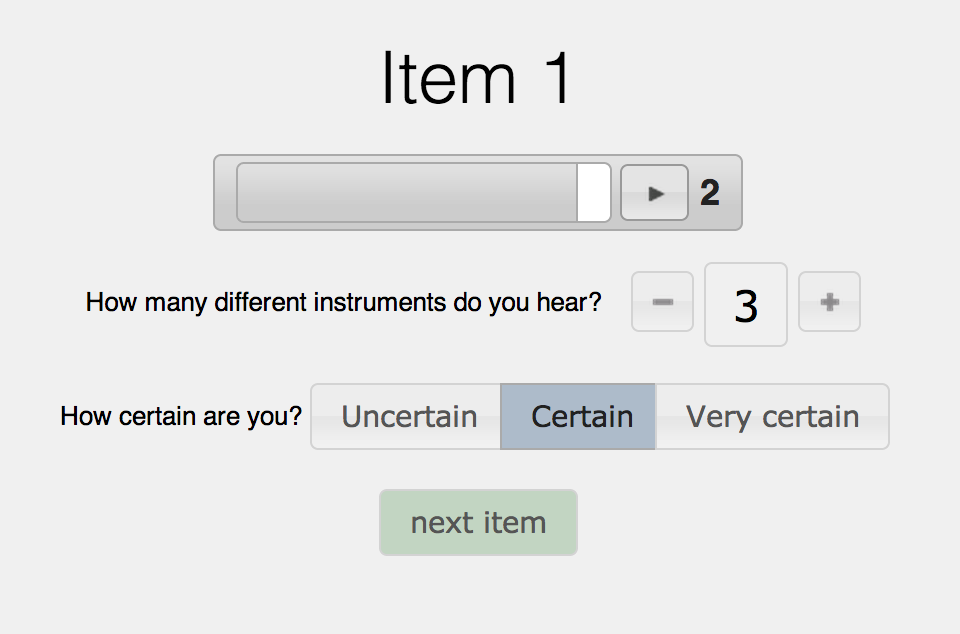
\includegraphics[width=2.8in]{Chapters/07_Analysis_Experiment/figures/user_interface.png}}
	\caption{Experiment User Interface.}
	\label{figure:user_interface}
\end{figure}

After the participants estimated the number of instruments for all twelve stimuli, they were given a score based on their performance. Besides their personal score, a percentile rank showed how each participant performed compared to all the other participants.

\section{Results}\label{sec:results}

The independent variables are the number of instruments being played back ($\textit{Num}_{\mathrm{Inst}}$), whether a participant is musical ($\textit{Musical}$), professional in audio ($\textit{Professional}$) and which setup was used ($\textit{Setup}$). A participant is defined as musical ($\textit{Musical} = true$) when he or she is regularly playing an instrument (including singing). The same applies to being professional ($\textit{Professional} = true$) which is set when the participant responded that he or she is a professional in audio. The responses for the setup used can either be headphones ($\textit{Setup} = \textrm{`}headphones\textrm{'}$) or loudspeaker ($\textit{Setup} = \textrm{`}loudspeaker\textrm{'}$). The dependent variable is the participant's estimation of the number of instruments being played back ($\textit{Resp}$). A correct estimation is defined as
\begin{equation}
\label{equation:response_correct}
\textit{Resp}_{\mathrm{Correct}} =
\begin{cases}
0 & \text{if } \text{\textit{Num}}_{\mathrm{Inst}} \neq \text{\textit{Resp}}
\\
1 & \text{if } \text{\textit{Num}}_{\mathrm{Inst}} = \text{\textit{Resp}}
\end{cases}
\mathrm{.}
\end{equation}
Table~\ref{table:responses} shows the responses of the participants for all stimuli.
\tabcolsep=5.5pt
\begin{table}[t]
\tiny
\begin{tabular}{p{1cm}ccccccc}
\toprule[1.5pt]
 & \multicolumn{ 7}{c}{$\textit{Num}_{\mathrm{Inst}}$} \\
  \cmidrule(l){2-8}
 $\textit{Resp}$ & $I=1$ & $I=2$ & $I=3$ & $ I=4$ & $I=5$ & $I=6$ & n \\

 \midrule
 $R=1$ & \cellcolor[gray]{0.9} 2025 & 373 & 5 & 18 & 13 & 12 & 2446 \\
 \midrule
 $R=2$ & 298 & \cellcolor[gray]{0.9} 1642 & 810 & 736 & 451 & 382 & 4319 \\
 \midrule
 $R=3$ & 12 & 277 & \cellcolor[gray]{0.9} 1343 & 1145 & 1093 & 1069 & 4939 \\
 \midrule
 $R=4$ & 1 & 43 & 158 & \cellcolor[gray]{0.9} 386 & 645 & 680 & 1913 \\
 \midrule
 $R=5$ & 0 & 1 & 18 & 48 & \cellcolor[gray]{0.9} 120 & 155 & 342 \\
 \midrule
 $R=6$ & 0 & 0 & 1 & 3 & 12 & \cellcolor[gray]{0.9} 30 & 46 \\
 \midrule
 $R>6$ & 0 & 0 & 1 & 0 & 2 & 8 & 11 \\

 \midrule
 & \multicolumn{7}{c}{14016 responses (1168 participants $\cdot$ 12 items)} \\
\midrule[1pt]

Probability of $\textit{Resp}_{\mathrm{Correct}}$ & 0.87 & 0.70 & 0.57 & 0.17 & 0.05 & 0.01 &  \\

 \bottomrule[1.5pt]
\end{tabular}
\caption{Responses from the participants. The cells with a gray background represent correct estimations.}
\label{table:responses}
\end{table}
\tabcolsep=6pt

For testing hypotheses, a logistic regression model with the response variable $\textit{Resp}_{\mathrm{Correct}}$ and the predictor variables $\textit{Num}_{\mathrm{Inst}}$, $\textit{Musical}$, $\textit{Professional}$ and $\textit{Setup}$ was calculated.
The estimated coefficients, p-values and average marginal effects are shown in Table~\ref{table:data_web_lm}.
\tabcolsep=5.5pt
\begin{table}[t]
\center
\scriptsize
\begin{tabular}{p{1.5cm}ccccp{0.8cm}}
\toprule[1.5pt]
Coefficient & Estimate & Std. Error & z-value & p-value & Average Marginal Effects \\
\midrule
(Intercept) & 1.5015 & 0.06836 & 21.963 & \textless~2e-16 & 0.1886 \\
$\textit{Num}_{\mathrm{Inst}} = 2$ & -1.0293 & 0.07651 & -13.453  & \textless~2e-16 & -0.1293\\
$\textit{Num}_{\mathrm{Inst}} = 3$ & -1.6021 & 0.07463 & -21.466  & \textless~2e-16 & -0.2012\\
$\textit{Num}_{\mathrm{Inst}} = 4$ & -3.5674 & 0.08380 & -42.572  & \textless~2e-16 & -0.4481\\
$\textit{Num}_{\mathrm{Inst}} = 5$ & -4.8759 & 0.11290 & -43.188  & \textless~2e-16 & -0.6125\\
$\textit{Num}_{\mathrm{Inst}} = 6$ & -6.3061 & 0.19428 & -32.459  & \textless~2e-16 & -0.7922\\
$\textit{Musical} = true$ & 0.5266 & 0.04932 & 10.676  & \textless~2e-16 & 0.0661\\
$\textit{Professional} = true$ & 0.3306 & 0.06234 & 5.303  & 1.14e-07 & 0.0415\\
$\textit{Setup} = \textrm{`}headphones\textrm{'}$ & 0.1071 & 0.04823 & 2.220  & 0.0264 & 0.0135\\
\midrule
\multicolumn{6}{l}{(Dispersion parameter for binomial family taken to be 1)}\\
\multicolumn{6}{l}{Null deviance: 18816  on 14015  degrees of freedom}\\
\multicolumn{6}{l}{Residual deviance: 11036  on 14007  degrees of freedom}\\
\multicolumn{6}{l}{AIC: 11054}\\
\multicolumn{6}{l}{Number of Fisher Scoring iterations: 7}\\
\multicolumn{6}{l}{McFadden's Pseudo R-squared: 0.413}\\
\bottomrule[1.5pt]
\end{tabular}
\tabcolsep=6pt
\caption{Logit regression model for response variable $\textit{Resp}_{\mathrm{Correct}}$ calculated from the data obtained by the Internet experiment.}
\label{table:data_web_lm}
\end{table}
Average marginal effects in the regression model describe the increase in probability for correctly estimating the number of instruments when the predictor variable is increased by one level. Compared to the other coefficients the average marginal effect of $\textit{Setup} = \textrm{`}headphones\textrm{'}$ is very low. By using headphones instead of loudspeakers it is $1.35\%$ more likely to estimate the number of instruments correctly.

As expected, participants who play an instrument or do singing ($\textit{Musical} = true$) performed slightly better than non-musicians. According to the average marginal effect their chance of estimating the number of instruments correctly is $6.61\%$ more likely for all stimuli. A similar increase for estimating the number correctly ($4.15\%$) can be seen for participants being a professional in audio ($\textit{Professional} = true$).

The average marginal effects of $\textit{Num}_{\mathrm{Inst}}$ indicates up to which point humans are able to correctly estimate the number of instruments being played back. The average marginal effect of $\textit{Num}_{\mathrm{Inst}} = 2$ shows that it is $12.93\%$ less likely to estimate correctly when listening to two instruments instead of one instrument. Furthermore, in case of three instruments being played back the probability of estimating the wrong number increases to $20.12\%$. The highly negative average marginal effect of $-0.4481$ for $\textit{Num}_{\mathrm{Inst}} = 4$ indicates that it is becoming very unlikely for humans to estimate the number of instruments correctly compared to estimating the number of one to three instruments.

For a detailed analysis of the differences between the Internet experiment and the laboratory experiment in a controlled environment, a second logit regression model was calculated. This logit regression model includes the data of the previous experiment which has responses of 62 participants. Besides $\textit{Num}_{\mathrm{Inst}}$ an additional predictor variable $\textit{Environment}$ was added which can have the values $\textrm{`}web\textrm{'}$ or $\textrm{`}lab\textrm{'}$ (described in Table~\ref{table:data_both_lm}).
\begin{table}[t]
\center
\scriptsize
\begin{tabular}{p{1.5cm}ccccp{0.8cm}}
\toprule[1.5pt]
Coefficient & Estimate & Std. Error & z-value & p-value & Average Marginal Effects \\
\midrule
(Intercept) & 2.0226 & 0.11718 & 17.260 & \textless~2e-16 & 0.2590\\
$\textit{Num}_{\mathrm{Inst}} = 2$ & -1.0135 & 0.07424 & -13.652  & \textless~2e-16 & -0.1298\\
$\textit{Num}_{\mathrm{Inst}} = 3$ & -1.5914 & 0.07223 & -22.033  & \textless~2e-16 & -0.2038\\
$\textit{Num}_{\mathrm{Inst}} = 4$ & -3.4786 & 0.08031 & -43.316  & \textless~2e-16 & -0.4454\\
$\textit{Num}_{\mathrm{Inst}} = 5$ & -4.8058 & 0.10919 & -44.015  & \textless~2e-16 & -0.6154\\
$\textit{Num}_{\mathrm{Inst}} = 6$ & -6.2481 & 0.19033 & -32.827  & \textless~2e-16 & -0.8000\\
$\textit{Environment} = \textrm{`}web\textrm{'}$ & -0.1435 & 0.10569 & -1.358  & 0.174 & -0.0184\\
\midrule
\multicolumn{6}{l}{(Dispersion parameter for binomial family taken to be 1)}\\
\multicolumn{6}{l}{Null deviance: 19826  on 14759  degrees of freedom}\\
\multicolumn{6}{l}{Residual deviance: 11819  on 14753  degrees of freedom}\\
\multicolumn{6}{l}{AIC: 11833}\\
\multicolumn{6}{l}{Number of Fisher Scoring iterations: 7}\\
\multicolumn{6}{l}{McFadden's Pseudo R-squared: 0.404}\\
\bottomrule[1.5pt]
\end{tabular}
\caption{Logit regression model for response variable $\textit{Resp}_{\mathrm{Correct}}$ calculated from the data obtained by the Internet experiment and the laboratory experiment.}
\label{table:data_both_lm}
\end{table}
The second logit regression model reveals that there are no significant differences ($p = 0.174$) between the two experiments. The low average marginal effect of $-0.0184$ also confirms that the type of the conducted experiments is applicable for an Internet environment.

Figure~\ref{figure:error_probability_iis_vs_web} depicts the mean probability for correctly estimating the number of instruments grouped by the environment. Since in \cite{Stoter2013} the differences between musicians and non-musicians were emphasized, their data is also depicted in Figure~\ref{figure:error_probability_iis_vs_web}.
\begin{figure}[t]
\centering
\begin{tikzpicture}

\begin{axis}[
xlabel={Number of Instruments},
ylabel={Mean of $\textit{Resp}_{\mathrm{Correct}}$},
legend style={
font=\tiny,
ymax=1.1,
legend pos=north east,
},
legend cell align=left
]

\addplot[color=red,mark=triangle,dash pattern=on 1pt off 1pt] plot file {Chapters/07_Analysis_Experiment/plotdata/error_prob_iis_musicians.data};
\addlegendentry{Musicians [lab]}

\addplot[color=blue,mark=o,dash pattern=on 1pt off 1pt] plot file {Chapters/07_Analysis_Experiment/plotdata/error_prob_iis_non_musicians.data};
\addlegendentry{Non-Musicians [lab]}

\addplot[color=black,mark=square,dash pattern=on 1pt off 1pt] plot file {Chapters/07_Analysis_Experiment/plotdata/error_prob_iis_all.data};
\addlegendentry{All [lab]}


\addplot[color=red,mark=triangle] plot file {Chapters/07_Analysis_Experiment/plotdata/error_prob_web_musicians.data};
\addlegendentry{Musicians [web]}

\addplot[color=blue,mark=o] plot file {Chapters/07_Analysis_Experiment/plotdata/error_prob_web_non_musicians.data};
\addlegendentry{Non-Musicians [web]}

\addplot[color=black,mark=square] plot file {Chapters/07_Analysis_Experiment/plotdata/error_prob_web_all.data};
\addlegendentry{All [web]}



\end{axis}
\end{tikzpicture}
\caption{Probability of $\textit{Resp}_{\mathrm{Correct}}$ grouped by Internet experiment (web) and laboratory experiment (lab). Solid lines represents the results of the Internet experiment and dashed lines represents the results of the laboratory experiment.}
\label{figure:error_probability_iis_vs_web}
\end{figure}
As the logit regression model indicated, the difference in the performance of the participants between the Internet experiment and the laboratory experiment are very low. The participants in the laboratory experiment were about 4.6\% better in average for all stimuli than the participants of the Internet experiment. When looking into the differences between musicians and non-musicians, the outcome for the Internet experiment and laboratory experiment differ slightly. In the laboratory experiment musicians performed about 31.6\% better than non-musicians and in the Internet experiment musicians performed about 20.85\% better.

The probability of correctly estimating the number of instruments does not consider how close an estimation is to the actual number of instruments. This means that a participant who estimates wrong by one instrument for all items has the same $\textit{Resp}_{\mathrm{Correct}}$ like a participant who is always wrong by two instruments. Despite this work focuses on the correct estimation, the differences in the absolute deviation to the correct number of instruments was also analyzed. The absolute deviation is defined as
\begin{equation}
\textit{Dev}_{\mathrm{Abs}} = | \textit{Num}_{\mathrm{Inst}} - \textit{Resp} |
\mathrm{.}
\label{equation:absolute_deviation}
\end{equation}
Figure~\ref{figure:absolute_deviation} depicts the mean of $\textit{Dev}_{\mathrm{Abs}}$ for the laboratory experiment and the Internet experiment. A knee point can be seen for $\textit{Num}_{\mathrm{Inst}} = 3$ where the slope of $\textit{Dev}_{\mathrm{Abs}}$ changes.

\begin{figure}[t]
\centering
\vspace{0.38cm}
\begin{tikzpicture}

\begin{axis}[
xlabel={Number of Instruments},
ylabel={Mean of Absolute Deviation},
legend style={
font=\tiny,
legend pos=north west,
},
legend cell align=left
]


\addplot[color=blue,mark=triangle,dash pattern=on 1pt off 1pt] plot file {Chapters/07_Analysis_Experiment/plotdata/mean_absolute_deviation_iis.data};
\addlegendentry{lab}

\addplot[color=red,mark=triangle] plot file {Chapters/07_Analysis_Experiment/plotdata/mean_absolute_deviation_web.data};
\addlegendentry{web}


\end{axis}
\end{tikzpicture}
\caption{The mean of the absolute deviation grouped by Internet Experiment (web) and laboratory experiment (lab).}
\label{figure:absolute_deviation}
\end{figure}

\makeatletter
\pgfplotstableread{Chapters/07_Analysis_Experiment/plotdata/share_very_certain.data}\tableA
\pgfplotstableread{Chapters/07_Analysis_Experiment/plotdata/share_certain.data}\tableB
\pgfplotstableread{Chapters/07_Analysis_Experiment/plotdata/share_uncertain.data}\tableC
\pgfplotsset{calculate offset/.code={\pgfkeys{/pgf/fpu=true,/pgf/fpu/output format=fixed}\pgfmathsetmacro\testmacro{(\pgfplotspointmeta*10^\pgfplots@data@scale@trafo@EXPONENT@y)/2*\pgfplots@y@veclength)}\pgfkeys{/pgf/fpu=false}},nodes near coords vertically centered/.style={every node near coord/.append style={/pgfplots/calculate offset,yshift=-\testmacro},nodes near coords align=center}}
\makeatother

\begin{figure}[t]
\centering
\vspace{2.5pt}

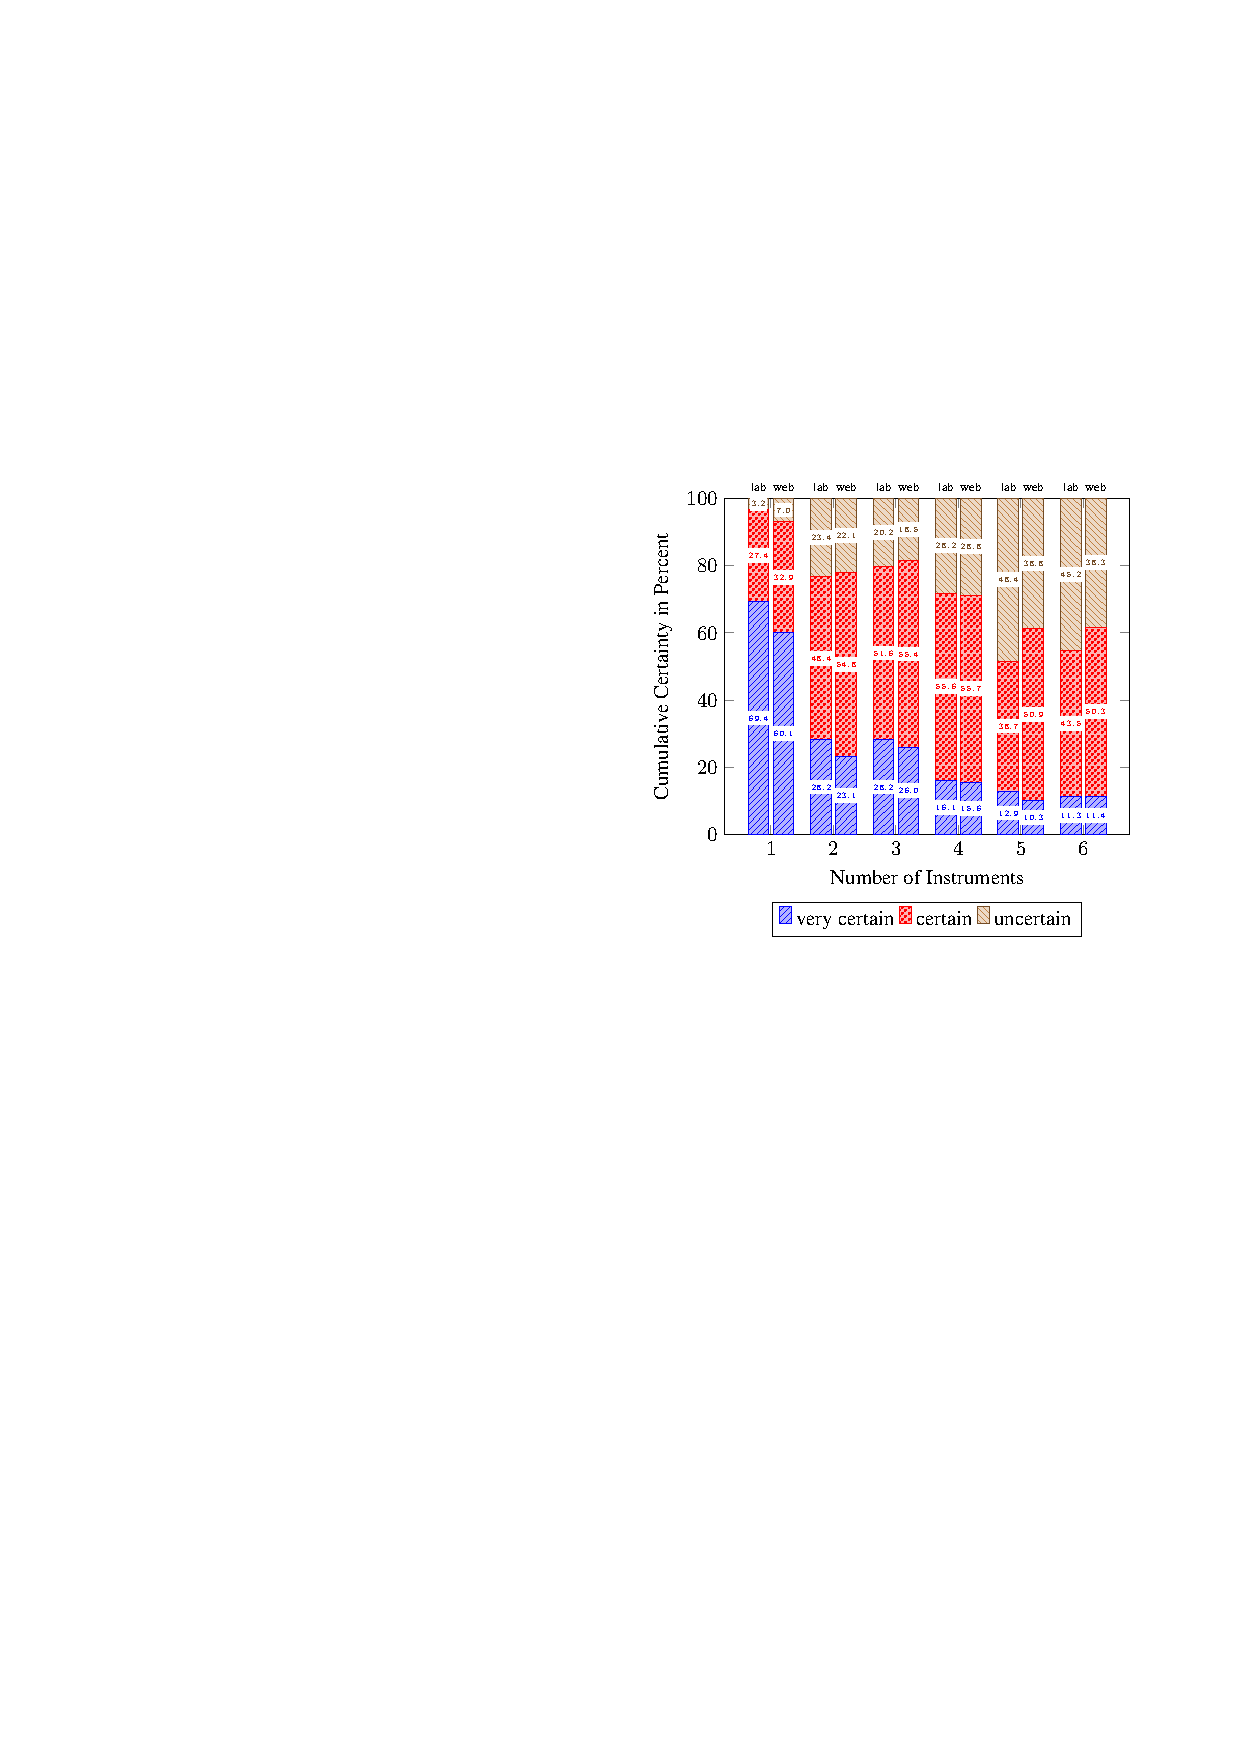
\includegraphics[width=0.45\textwidth]{Chapters/07_Analysis_Experiment/plotdata/certainty.pdf}
\caption{Differences in certainty between the Internet experiment (web) and laboratory experiment (lab).}
\label{figure:certainty_web_iis}
\end{figure}

To confirm the marginal differences between the Internet experiment and laboratory experiment for $\textit{Dev}_{\mathrm{Abs}}$, a linear regression model was calculated.
The result tables can be found in~\cite{schoeffler13}.
% \begin{table}[h]
% \center
% \scriptsize
% \begin{tabular*}{0.45\textwidth}{p{1.5cm}ccccp{0.8cm}}
% \toprule[1.5pt]
% Coefficient & Estimate & Std. Error & z-value & p-value\\
% \midrule
% (Intercept) & 0.08535 & 0.02706 & 3.154 & 0.00161\\
% $\textit{Num}_{\mathrm{Inst}} = 2$ & 0.17683 & 0.01881 & 9.401  & \textless~2e-16\\
% $\textit{Num}_{\mathrm{Inst}} = 3$ & 0.30122 & 0.01881 & 16.014  & \textless~2e-16\\
% $\textit{Num}_{\mathrm{Inst}} = 4$ & 1.02154 & 0.01881 & 54.309  & \textless~2e-16\\
% $\textit{Num}_{\mathrm{Inst}} = 5$ & 1.67967 & 0.01881 & 89.297  & \textless~2e-16\\
% $\textit{Num}_{\mathrm{Inst}} = 6$ & 2.56667 & 0.01881 & 136.453  & \textless~2e-16\\
% $\textit{Environment} = \textrm{`}web\textrm{'}$ & 0.05481 & 0.02482 & 2.208  & 0.02724\\
% \midrule
% \multicolumn{5}{l}{Residual standard error: 0.6597 on 14753 degrees of freedom}\\
% \multicolumn{5}{l}{Multiple R-squared: 0.6603,	Adjusted R-squared: 0.6602}\\
% \multicolumn{5}{l}{F-statistic:  4779 on 6 and 14753 DF,  p-value: \textless~2.2e-16}\\
% \bottomrule[1.5pt]
% \end{tabular*}
% \caption{Linear regression model for $\textit{Dev}_{\mathrm{Abs}}$ calculated from the data obtained by the Internet experiment and the laboratory experiment.}
% \label{table:lm_absolute_deviation}
% \end{table}

Another response variable that was obtained from the participants was the certainty of their estimation. Figure~\ref{figure:certainty_web_iis} depicts the certainty values for the Internet experiment and the laboratory experiment.

For testing whether the environment has a significant influence on the certainty of the participants ($\textit{Certainty}$), a cumulative link model (also called ordered regression model) was calculated\cite{Christensen2012}. The cumulative link model is used since $\textit{Certainty}$ is an ordered dependent variable with the possible values `uncertain', `certain' and `very certain'. The predictor variables for the ordered regression model are $\textit{Num}_{\mathrm{Inst}}$ and $\textit{Environment}$. Again, the details of the cumulative link model for $\textit{Certainty}$ can be found in~\cite{schoeffler13}.

% \begin{table}[t]
% \center
% \scriptsize
% \begin{tabular*}{0.45\textwidth}{cccccc}
% \toprule[1.5pt]
% Coefficient & Estimate & Std. Error & z-value & p-value\\
% \midrule
% $\textit{Num}_{\mathrm{Inst}} = 2$ & -1.61273 & 0.05744 & -28.078  & \textless~2e-16\\
% $\textit{Num}_{\mathrm{Inst}} = 3$ & -1.43164 & 0.05701 & -25.114  & \textless~2e-16\\
% $\textit{Num}_{\mathrm{Inst}} = 4$ & -2.02315 & 0.05804 & -34.858  & \textless~2e-16\\
% $\textit{Num}_{\mathrm{Inst}} = 5$ & -2.47933 & 0.05901 & -42.013  & \textless~2e-16\\
% $\textit{Num}_{\mathrm{Inst}} = 6$ & -2.43573 & 0.05900 & -41.283  & \textless~2e-16\\
% $\textit{Environment} = \textrm{`}web\textrm{'}$ & -0.01008 & 0.07355 & -0.137  & 0.891\\
% \midrule
% \multicolumn{5}{l}{Threshold coefficients:}\\
% & Estimate & Std. Error & z-value &\\
% $uncertain|certain$ & -2.90465 & 0.08434 & -34.441  &\\
% $certain|very certain$ & -0.41072 & 0.08090 & -5.077  &\\
% \multicolumn{5}{l}{AIC: 28242.52}\\
% \bottomrule[1.5pt]
% \end{tabular*}
% \caption{Logit cumulative link model of certainty that was calculated from the data obtained by the Internet experiment and the laboratory experiment.}
% \label{table:olr_both}
% \end{table}
% Same as $\textit{Resp}_{\mathrm{Correct}}$, the environment of the experiment has no significant influence on the dependent variable $\textit{Certainty}$. Considering the number of participants and the comparable low coefficient, the environment had a very low influence on $\textit{Certainty}$.

\vspace{-0.1in}
\section{Discussion}\label{sec:discussion}

Regarding the ability of estimating the number of instruments, the web experiment confirmed the results of the laboratory experiment\cite{Stoter2013}. Both experiments share the same outcome: The probability to correctly estimate up to about three instruments is higher than 50\%.

In our previous result analysis of the laboratory experiment\cite{Stoter2013} we set the focus on the differences between musicians and non-musicians. Between the Internet experiment and the laboratory experiment, slightly different results were obtained when looking into how musicians and non-musicians performed (Figure~\ref{figure:error_probability_iis_vs_web}). In the laboratory experiment musicians performed much better compared to non-musicians than in the Internet Experiment. One reason seems to be that in the laboratory experiment 74.2\% of the musicians had also a professional background in audio. In the Internet experiment only 27.5\% of the musicians had a professional background in audio. Since audio professionals more often have to detect hardly audible differences in audio files they are more trained in this field. As mentioned before, being a musician in our context does just mean that the participant plays an instrument without any information about his expert level or the time he or she spends on practicing.

When examining the responses for items with the same number of instruments being played back, noticeable differences between the genres were found. For the stimuli with $\textit{Num}_{\mathrm{Inst}} \le 4$ the mean of $\textit{Resp}_{\mathrm{Correct}}$ was $53.0\%$ and for non-classical items $62.5\%$. Since the experiment was not designed for testing classical versus non-classical items, we cannot make definitive statements about whether humans are better in estimating instruments for a specific music genre. Moreover, we did not address this issue in our result analysis.

One of the main reasons for conducting the experiment was to find out which influence the Internet environment has on the results. All three regression models which included data of both experiments revealed that the Internet environment had only very minor effects on the results. Moreover, despite the large number of participants in both experiments, the predictor variable $\textit{Environment}$ was even not significant in two out of three regression models.

It is often recommended to use headphones instead of loudspeakers for Internet experiments. From the relative low average marginal effect of $\textit{Setup}$ (Table~\ref{table:data_web_lm}), it can be derived that the type of the setup had only minor effects on the results of the Internet experiment.

Surprising was the small number of participants who had to be screened. We excluded 27 participants since they gave at least one non-serious response which is about 2.3\% (1195 participants remained after excluding all trials which were not the first ones). Most of these excluded participants responded with either very high numbers (e.~g. 99) or responded with zeros for their estimated number of instruments being played. We assume that especially participants who responded with zero only wanted to get an impression of the experiment.

\section{Exeriment on Speaker Count Estimation}

\begin{figure}[htb]
	\centering
		\fbox{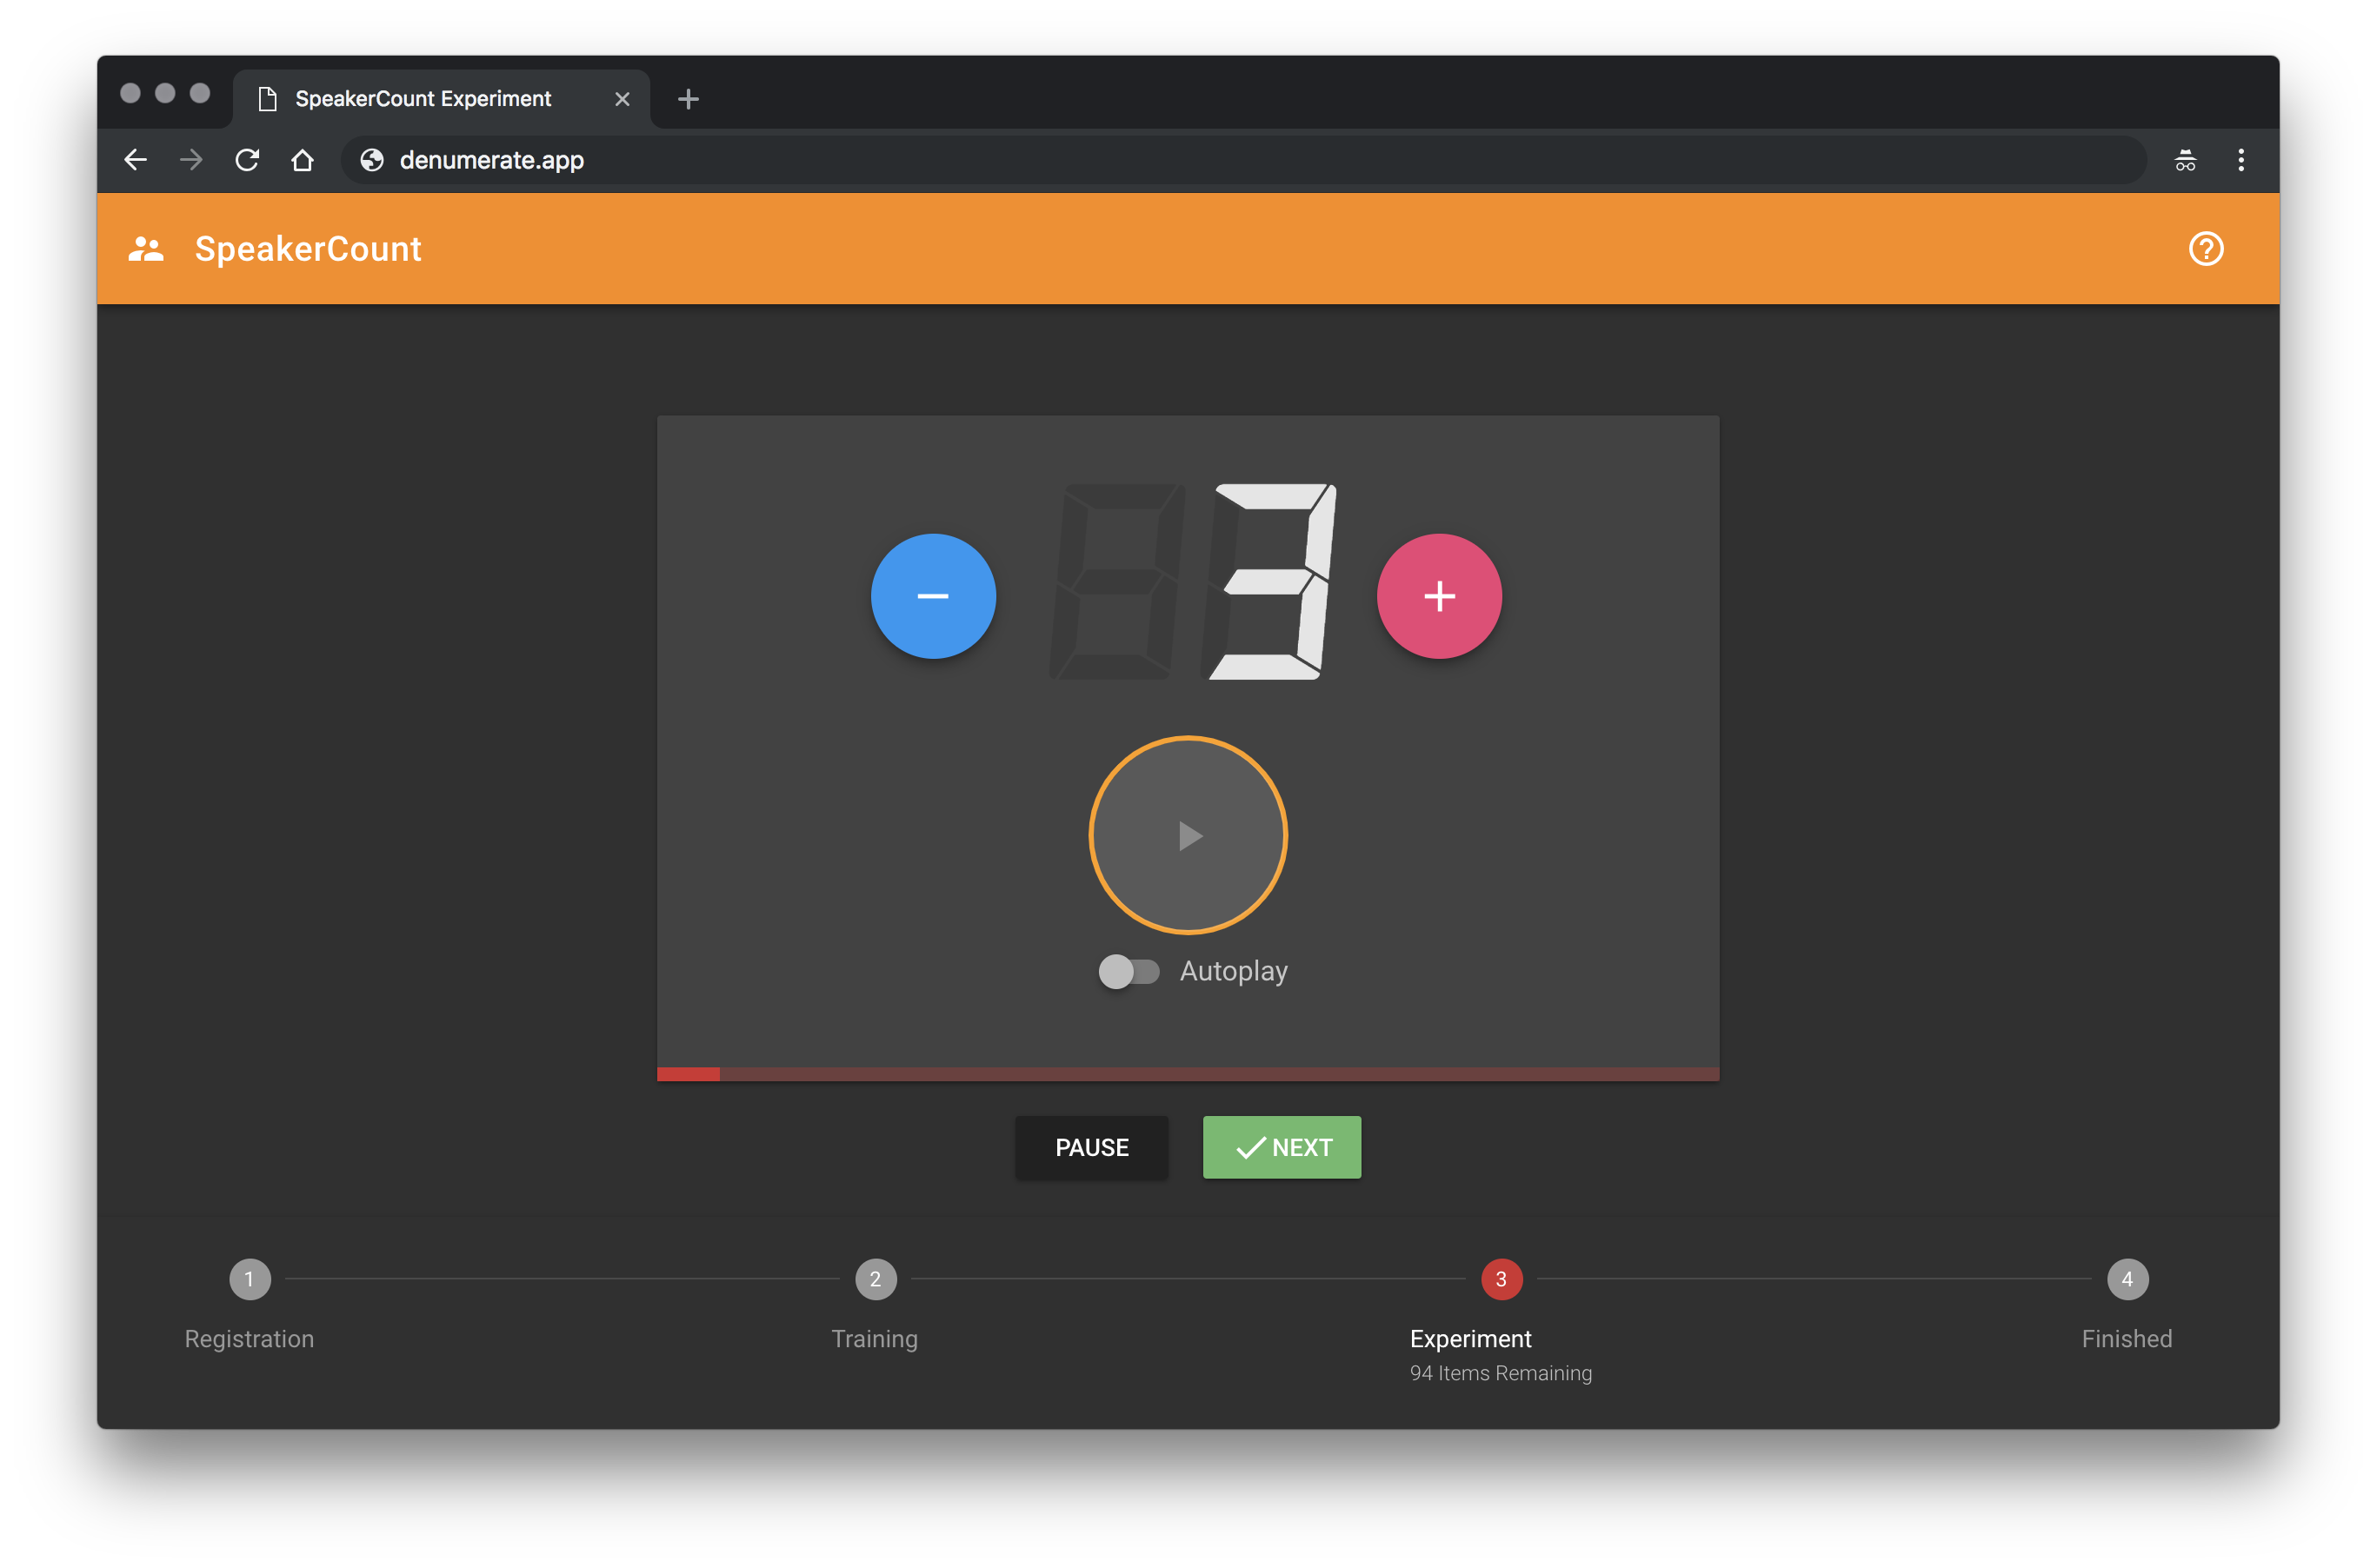
\includegraphics[width=0.8\textwidth]{Chapters/07_Analysis_Experiment/figures/experiment_ui.png}}
	\caption{Experiment User Interface.}
	\label{fig:user_interface}
\end{figure}

In a ``cocktail-party'' scenario, one or more microphones capture the signal from many concurrent speakers. In this setting, different applications may be envisioned such as localization, crowd monitoring, surveillance, speech recognition, speaker separation, etc.
When devising a system for such a task, it is typically assumed that the actual number of concurrent speakers is known.
This assumption turns out to be of paramount importance for the effectiveness of subsequent processing.
Notably, for separation algorithms~\cite{common10},
real-world systems do not straightforwardly provide information about the actual number of concurrent speakers.
\par
When speaker overlap is as prevalent as in a ``cocktail-party'' scenario, developing an algorithm to detect the number of speakers is challenging.
This is in contrast to humans whom we know are excellent in segregating one source from a mixture~\cite{bregman} and tend to use this skill to perceptually segregate speakers before they can estimate a count, as highlighted, e.g.\ in~\cite{kawashima15}.
As shown in~\cite{kashino96, kawashima15}, humans are able to correctly estimate up to three simultaneously active speakers without using spatial information.
Similarly, in music, psycho-acoustic researchers came up with a ``one-two-three-many'' hypothesis~\cite{huron89, stoeter13, schoeffler13}.
The question if machines could outperform humans, or if they are subject to similar limitations, remains to be answered.
%
\par
Identifying isolated sources in realistic mixtures is challenging~\cite{bregman} and psychology studies in vision~\cite{jevons1871} have shown that humans can instantly estimate the number of objects without actually counting and therefore identifying them.
This phenomenon is known as \textit{subitizing} and has been inspiring research in vision~\cite{chattopadhyay17}.
Since there are indications that the auditory system is also capable of subitizing sources~\cite{hoopen79}, we transfer this fact to the audio domain and directly attempt in this study to estimate the number of audio sources instead of counting them after identification.
We refer to this strategy as ``direct count estimation''.

% * Reference existing listening tests which report the same thing
% * Are we really doing it? We can decide on this once the first full draft is ready.
In a first step, we chose to reproduce the experiments made in~\cite{kawashima15, kashino96}.
Kawashima et al.\ found in extensive experiments using Japanese speech samples, that participants were able to correctly estimate up to three simultaneously active speakers without using any spatial cues.
We conducted our own study using the simulated data from the \emph{LIBRI Speech} (power normalized) data set.
We therefore randomly selected 10 samples for each \(k \in [0, \ldots, 10]\), resulting in 100 mixtures of 5~seconds duration each.
The experiment was done using \emph{between-group design}, where one group (blind experiment) did not get any prior information about the maximum number of speakers in the test set (similar to~\cite{kawashima15}).
However, the maximum number of speakers was revealed to the other group (informed experiment), which is more related to our data-driven, classification based CRNN.
Further, none of the participants received any feedback about the error made during the trials.
Similarly to~\cite{kawashima15}, lab-based experiments were conducted with ten participants for each group (\(n=20\)) using a custom designed web-based software.\footnote{The experiment is made available through the accompanying website.}
In all previous experiments, we used the mean absolute error metric which does not reveal over and underestimation errors.
We therefore decided to report the average response for each group of \(k\).
The results of our lab-based experiments are shown in Figure~\ref{fig:experiment}.
The results for up to three speakers indicate that humans perform similarly (or better in terms of variance) compared to our proposed CRNN model.
Results of the blind experiment show that underestimation becomes apparent for \(k > 3\).
As a reference, we also included the average results from~\cite{kawashima15} (Experiment 1, 5~seconds durations) which shows similar results compared to our blind experiment.
For larger speaker counts, the gap between humans and algorithm is almost three speakers on average.
Interestingly, the results of the informed experiment reveal that this gap closes down to an average difference of one speaker.
Finally, we can report that the machine model reached superhuman performance.
Unlike humans, the CRNN is subject to over-estimations for \(4 < k \leq 9\).
However, with extensive training, humans might be able to perform on par.
When we asked participants about the strategy they pursued, many reported that with more than three speakers it is not possible to identify (and count) the speakers but rather compare the \emph{density} of the speech to that of 1-3 speakers.
For higher speaker counts, participants reported that the integrated phoneme activity was a relevant cue, supporting our previously mentioned hypothesis.

\begin{figure}[t!]
    \centering
    \begin{adjustbox}{width=0.7\columnwidth}
      % This file was created by matplotlib2tikz v0.6.13.
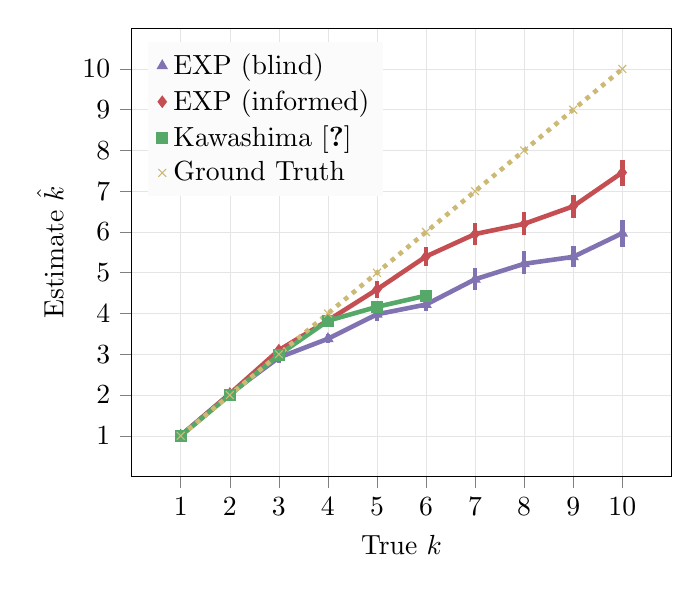
\begin{tikzpicture}

\definecolor{color1}{rgb}{0.298039215686275,0.447058823529412,0.690196078431373}
\definecolor{color0}{rgb}{0.917647058823529,0.917647058823529,0.949019607843137}
\definecolor{color4}{rgb}{0.768627450980392,0.305882352941176,0.32156862745098}
\definecolor{color2}{rgb}{0.333333333333333,0.658823529411765,0.407843137254902}
\definecolor{color5}{rgb}{0.8,0.725490196078431,0.454901960784314}
\definecolor{color3}{rgb}{0.505882352941176,0.447058823529412,0.698039215686274}

\begin{axis}[
xlabel={True \(k\)},
ylabel={Estimate \(\hat{k}\)},
xmin=-1, xmax=10,
ymin=0, ymax=11,
ytick={1,2,3,4,5,6,7,8,9,10},
xtick={0,1,2,3,4,5,6,7,8,9},
xticklabels={1,2,3,4,5,6,7,8,9,10},
tick align=outside,
tick pos=left,
ymajorgrids,
xmajorgrids,
grid style={line width=.1pt, draw=gray!20},
major grid style={line width=.2pt,draw=gray!20},
axis line style={black},
legend style={at={(0.03,0.97)}, anchor=north west, draw=none, fill=color0!20},
legend cell align={left},
legend entries={{EXP (blind)}, {EXP (informed)}, {Kawashima~\cite{kawashima15}}, {Ground Truth}}
]

\addplot [only marks, mark size=2.0, mark=triangle*, draw=color3, fill=color3, colormap/blackwhite]
table{%
x                      y
+0.000000000000000e+00 +1.010000000000000e+00
+1.000000000000000e+00 +2.030000000000000e+00
+2.000000000000000e+00 +2.920000000000000e+00
+3.000000000000000e+00 +3.380000000000000e+00
+4.000000000000000e+00 +3.980000000000000e+00
+5.000000000000000e+00 +4.220000000000000e+00
+6.000000000000000e+00 +4.840000000000000e+00
+7.000000000000000e+00 +5.220000000000000e+00
+8.000000000000000e+00 +5.390000000000000e+00
+9.000000000000000e+00 +5.970000000000000e+00
};
\addplot [line width=1.66pt, color3, forget plot]
table {%
0 1.01
1 2.03
2 2.92
3 3.38
4 3.98
5 4.22
6 4.84
7 5.22
8 5.39
9 5.97
};
\addplot [line width=1.66pt, color3, forget plot]
table {%
0 1
0 1.03
};
\addplot [line width=1.66pt, color3, forget plot]
table {%
1 2
1 2.07
};
\addplot [line width=1.66pt, color3, forget plot]
table {%
2 2.78975
2 3.05
};
\addplot [line width=1.66pt, color3, forget plot]
table {%
3 3.27
3 3.5
};
\addplot [line width=1.66pt, color3, forget plot]
table {%
4 3.80975
4 4.16025
};
\addplot [line width=1.66pt, color3, forget plot]
table {%
5 4.06
5 4.4
};
\addplot [line width=1.66pt, color3, forget plot]
table {%
6 4.58
6 5.11
};
\addplot [line width=1.66pt, color3, forget plot]
table {%
7 4.97
7 5.53
};
\addplot [line width=1.66pt, color3, forget plot]
table {%
8 5.13
8 5.66
};
\addplot [line width=1.66pt, color3, forget plot]
table {%
9 5.64
9 6.29
};
\addplot [only marks, mark size=2.0, mark=diamond*, draw=color4, fill=color4, colormap/blackwhite]
table{%
x                      y
+0.000000000000000e+00 +1.000000000000000e+00
+1.000000000000000e+00 +2.030000000000000e+00
+2.000000000000000e+00 +3.100000000000000e+00
+3.000000000000000e+00 +3.830000000000000e+00
+4.000000000000000e+00 +4.590000000000000e+00
+5.000000000000000e+00 +5.400000000000000e+00
+6.000000000000000e+00 +5.950000000000000e+00
+7.000000000000000e+00 +6.200000000000000e+00
+8.000000000000000e+00 +6.630000000000000e+00
+9.000000000000000e+00 +7.460000000000000e+00
};
\addplot [line width=1.66pt, color4, forget plot]
table {%
0 1
1 2.03
2 3.1
3 3.83
4 4.59
5 5.4
6 5.95
7 6.2
8 6.63
9 7.46
};
\addplot [line width=1.66pt, color4, forget plot]
table {%
0 1
0 1
};
\addplot [line width=1.66pt, color4, forget plot]
table {%
1 1.97
1 2.1
};
\addplot [line width=1.66pt, color4, forget plot]
table {%
2 3
2 3.21
};
\addplot [line width=1.66pt, color4, forget plot]
table {%
3 3.67
3 3.98
};
\addplot [line width=1.66pt, color4, forget plot]
table {%
4 4.39
4 4.8
};
\addplot [line width=1.66pt, color4, forget plot]
table {%
5 5.16
5 5.64
};
\addplot [line width=1.66pt, color4, forget plot]
table {%
6 5.69
6 6.23
};
\addplot [line width=1.66pt, color4, forget plot]
table {%
7 5.91975
7 6.48
};
\addplot [line width=1.66pt, color4, forget plot]
table {%
8 6.34
8 6.92
};
\addplot [line width=1.66pt, color4, forget plot]
table {%
9 7.14
9 7.76025
};

\addplot [only marks, mark size=2.0, mark=square*, draw=color2, fill=color2, colormap/blackwhite]
table{%
x                      y
+0.000000000000000e+00 +1.000000000000000e+00
+1.000000000000000e+00 +2.000000000000000e+00
+2.000000000000000e+00 +2.987442378071903e+00
+3.000000000000000e+00 +3.821715111593599e+00
+4.000000000000000e+00 +4.163430371330779e+00
+5.000000000000000e+00 +4.438511376242037e+00
};
\addplot [line width=1.66pt, color2, forget plot]
table {%
0 1
1 2
2 2.9874423780719
3 3.8217151115936
4 4.16343037133078
5 4.43851137624204
};


\addplot [only marks, mark size=2.0, draw=color5, mark=x, fill=color5, colormap/blackwhite]
table{%
x                      y
+0.000000000000000e+00 +1.000000000000000e+00
+1.000000000000000e+00 +2.000000000000000e+00
+2.000000000000000e+00 +3.000000000000000e+00
+3.000000000000000e+00 +4.000000000000000e+00
+4.000000000000000e+00 +5.000000000000000e+00
+5.000000000000000e+00 +6.000000000000000e+00
+6.000000000000000e+00 +7.000000000000000e+00
+7.000000000000000e+00 +8.000000000000000e+00
+8.000000000000000e+00 +9.000000000000000e+00
+9.000000000000000e+00 +1.000000000000000e+01
};
\addplot [line width=1.66pt, color5, dotted, forget plot]
table {%
0 1
1 2
2 3
3 4
4 5
5 6
6 7
7 8
8 9
9 10
};
\end{axis}

\end{tikzpicture}

    \end{adjustbox}
    \caption{Average responses from humans (\
    {EXP} and \emph{Kawashima}
~\cite{kawashima15}) compared to our proposed CRNN. Error bars show 95\% confidence intervals.}%
    \label{fig:experiment}
 \end{figure}
 % TODO add mean absolute error

 \section{Discussion and Scope}

\begin{itemize}
  \item More stimulus instead of more participants to train a dnn to match human performance.
  \item good task for a web based experiment.
\end{itemize}
